\documentclass[pdftex,12pt,a4paper]{article}

\usepackage{graphicx}  
\usepackage[margin=2.5cm]{geometry}
\usepackage{breakcites}
\usepackage{indentfirst}
\usepackage{pgfgantt}
\usepackage{pdflscape}
\usepackage{float}
\usepackage{epsfig}
\usepackage{epstopdf}
\usepackage[cmex10]{amsmath}
\usepackage{stfloats}
\usepackage{multirow}

\renewcommand{\refname}{REFERENCES}
\linespread{1.3}

% REQUIRED FOR INSETYING SOME SHITASS ASSEMBLY CODE INTO TO LATEX BIATCH fuck this retarded thing, science my ass
\usepackage{listings}
\usepackage{xcolor}
\definecolor{codegreen}{rgb}{0,0.6,0}
\definecolor{codegray}{rgb}{0.5,0.5,0.5}
\definecolor{codepurple}{rgb}{0.58,0,0.82}
\definecolor{backcolthe}{rgb}{0.95,0.95,0.92}
\definecolor{CommentGreen}{rgb}{0,.6,0}
% bu salak seyin son satiri bosluk olunca calismiyor kendimi sikcem simdi
% Icine comment de konmuyor

\lstset{
    numbers=left,
    basicstyle=\small\ttfamily,
    numberstyle=\tiny,
    keywordstyle=\color{blue}\bfseries,
    keywordsprefix=B,
    language={[x86masm]Assembler},
    breaklines=true,
    commentstyle=\color{codegreen},
    keywordstyle=\color{blue},
    keywordstyle=[2]\color{orange},
    keywordstyle=[3]\color{codegray},
    numberstyle=\tiny\color{codegray},
    stringstyle=\color{codepurple},
    showtabs=false,
    frame=single,
    keepspaces,
}



\usepackage{mathtools}
%\newcommand{\HRule}{\rule{\linewidth}{0.5mm}}
\thispagestyle{empty}
\begin{document}
\begin{titlepage}
\begin{center}
\textbf{}\\
\textbf{\Large{ISTANBUL TECHNICAL UNIVERSITY}}\\
\vspace{0.5cm}
\textbf{\Large{COMPUTER ENGINEERING DEPARTMENT}}\\
\vspace{2cm}
\textbf{\Large{BLG 351E\\ MICROCOMPUTER LABORATORY\\ EXPERIMENT REPORT}}\\
\vspace{2.8cm}
\begin{table}[ht]
\centering
\Large{
\begin{tabular}{lcl}
\textbf{EXPERIMENT NO}  & : & 7-8 \\
\textbf{EXPERIMENT DATE}  & : & 04.12.2019 \\
\textbf{LAB SESSION}  & : & WEDNESDAY - 13.30 \\
\textbf{GROUP NO}  & : & G10 \\
\end{tabular}}
\end{table}
\vspace{1cm}
\textbf{\Large{GROUP MEMBERS:}}\\
\begin{table}[ht]
\centering
\Large{
\begin{tabular}{rcl}
150170062  & : & Mehmet Fatih YILDIRIM \\
150180704  & : & Cihat AKK\.{I}RAZ \\
150180705  & : & Batuhan Faik DER\.{I}NBAY \\
150180707  & : & Fatih ALTINPINAR \\
\end{tabular}}
\end{table}
\vspace{2.8cm}
\textbf{\Large{FALL 2019-2020}}

\end{center}

\end{titlepage}

\newpage


\thispagestyle{empty}
\addtocontents{toc}{\contentsline {section}{\numberline {}FRONT COVER}{}}
\addtocontents{toc}{\contentsline {section}{\numberline {}CONTENTS}{}}
\setcounter{tocdepth}{4}
\tableofcontents
\clearpage

\setcounter{page}{1}


\section{INTRODUCTION}

In this experiment, 16x2 Dot-matrix LCD display and a random generator is implemented. While doing this implementation, experience and knowledge from old experiments are used. Also given informations and codes are used to understand how manipulating LCD display via using MSP430G2553 microcontroller.

\section{MATERIALS AND METHODS}

This experiment is conducted via using MSP430G2553 microprocessor. This microprocessor is programmed using Code Composer Studio according to desired tasks on the experiment handout. During coding below sources are used:

\begin{itemize}
    \item MSP430 Education Board Manual \cite{ref2}
    \item MSP430 Architecture Chapter 4 \cite{ref3}
    \item MSP430 Instruction Set \cite{ref4}
    \item Supplementary Chapter 6 General Purpose \cite{ref5}
    \item MSP430 User Guide - Chapter 8 \cite{ref5}
\end{itemize}

\subsection{Part 1}

In the first part of the experiment, the team was asked to implement a print function which uses char arrays (See Figure \ref{code:lcd-array}) as inputs and show them on the LCD display. Also while displaying this array, it is asked that \textbackslash{n} and \textbackslash{0} characters should be interpreted and create outputs according to these interpretations. (See Figure \ref{fig:output-lcd}).

\begin{figure}[H]
    \centering
    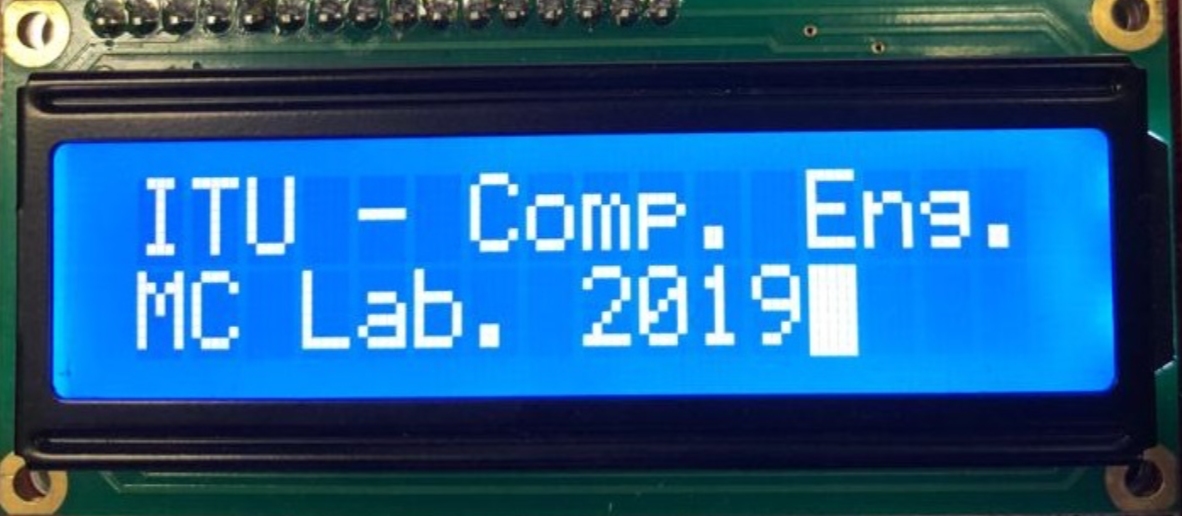
\includegraphics[width=0.5\textwidth]{output_lcd.png}
    \caption{Display on the 16x2 lcd asked string}
    \label{fig:output-lcd}
\end{figure}

\begin{figure}[H]
    \centering
    \begin{lstlisting}[language={[x86masm]Assembler}]
	.data
string 	.byte "ITU - Comp. Eng.",0Dh,"MC Lab. 2019",00h
    \end{lstlisting}
    \label{code:lcd-array}
    \caption{String asked to display on the LCD}
\end{figure}

To display and manipulate values on the LCD display, some configurations should be made. In these experiments, aforementioned configurations are already given to the team and the code for only to send data and display string on the LCD was asked. Given subroutines are listed below and the codes of these subroutines are not included in the report. In this report, only the parts of the code that are written by the team are included.

\begin{enumerate}
    \item initLCD
    \item sendCMD
    \item sendDATA (This part was edited by the team)
    \item delay
    \item trigerEN
\end{enumerate}

Let us go through the code and analyze the implementation.

\begin{itemize}
    \item Line 1: Address of string is moved to R10.
    \item Line 2-3: Controlling whether end of the line for current char. If the current element is '#0dh' jump to execute newline subroutine.
    \item Line 4-5: Controlling whether end of the sequence for current char. If the current element is '#00h' jump to execute endseq subroutine.
    \item Line 6-7: Moving char value on the R10 register to R5 for SendData subroutine and calling these subroutine.
    \item Line 8-9: Delay for sending data to LCD.
    \item Line 10-11: Incrementing R10 to process next char in the string array and jumping to beginning of the loop to process it.
    \item Line 13: Point to next character in the array.
    \item Line 14-15: Load the command for newline in R5 and send it.
    \item Line 16-18: Wait for the execution of newline operation, then return back to main loop.
    \item Line 20: Ends the sequence by jumping to infinite loop stop.
    \item Line 22: Puts the device in write mode so device is ready for receiving data.
    \item Line 23-30: Sends the upper nibble first then shifts the data 4 times and sends the second nibble.
    \item Line 31-32: Puts the device in read mode since no more data will be sent in the given function. Then returns from subroutine.
    \item Line 34-36: Infinite stop loop. Calls itself every 100 microseconds.
\end{itemize}
\begin{figure}[H]
    \centering
    \begin{lstlisting}[language={[x86masm]Assembler}]
		mov.w #string,	R10
loop		cmp.b   #0dh,	0(R10)
		jz	newline
		cmp.b	#00h,	0(R10)
		jz	endseq
		mov.b	@R10, R5
		call 	#SendData
		mov     &Delay100us, R15
		call 	#Delay
		add.w	#01b,	R10
		jmp loop

newline		add.w	#01b,	R10
		mov.b	#011000000b, R5
		call 	#SendCMD
		mov 	&Delay100us, R15
		call 	#Delay
		jmp		loop

endseq		jmp stop

SendData 	bis.b #080h,  &P2OUT
		mov.b R5, &P1OUT
		call #TrigEn
		rla R5
		rla R5
		rla R5
		rla R5
		mov.b R5, &P1OUT
		call #TrigEn
		bic.b 	#080h,	&P2OUT
		ret

stop 		mov.b	&Delay100us,	R15
		call #Delay
		jmp stop    \end{lstlisting}
    \label{code:part1_0123}
    \caption{Sending Data to the LCD Display - Part 1}
\end{figure}

%%%%%%%%%%%%%%%%%%%%%%%
\newpage
\subsection{Part 2}

In this part, a random generator is implemented and generated values are displayed on the 16x2 LCD dot display.

To accomplish this task the parts added or modified can be explained as following.

\begin{itemize}
    \item Line 6: Rather ending the sequence when $00h$ character received, program jumps to subroutine called $writenumber$ which will print the number on the LCD display.
    \item Line 89-120: In the interrupt service routine, following calculations are made to obtain a random number on $R9$. $R11$ holds the seed value, $R13$ is $x$ and $R10 = w$.
    \item Line 91-96: Taking square of the $x$ is done by calling multiplication subroutine by giving parameters as $x$ and $x$ again. Which returns $x^2$.
    \[x = square(x)\]
    \item Line 98-100: \(x = x +(w = w + s)\) is implemented by these lines. It sums the corresponding registers in order to obtain $x$ value.
    \item Line 101-110: \(r = (x>>4) | (x<<4)\) is calculated by using a temporary register $R6$ which was pushed to stack at the beginning of the interrupt service routine.
    \item Line 113: Increasing seed which is not an ideal thing to be done in order to obtain random numbers.
    \item Line 115: Sets $R12$. This register is checked in the stop sequence. If a new number comes system start to write to the LCD all over again.
    \item Line 117-120: Popping temporary register to its previous value and returning from interrupt.
    \item Line 22-56: In order to print the random number in $R9$, every digit has to be converted to character at first. This is done as following:
    \begin{itemize}
        \item Line 23-28: Finding hundreds digit by dividing $R9$
        by $100$. Result is going to be hold on $R7$.
        \item Line 30-43: Tens digit is found by the formula given below. This value is then loeaded to $R7$: \[TensDigit = RandomNumber / 10 - HundredsDigit \times 10\]
        \item Line 44-54: Units digit is found by the same way, then it is stored inside $R8$.
        \[UnitsDigit = RandomNumber - HunderdsDigit \times 100 - TensDigit \times 10\]
        \item Line 54-56: The numbers of every digit is found but these numbers have to be converted to char from int. Since LCD display uses ASCII, $48$ which is the value of ASCII $0$ is added to every register. This ensures all registers will have corresponding char values to be printed.
        \item Line 57-68: Digit by digit all numbers printed on the screen
    \end{itemize}
    \item Line 72-82: Enables $RS$ which allows data transmission. $R5$ is loaded with the data then LCD Display is triggered. Which takes upper nibble then lower. $R5$ shifted towards left in order to send lower nibble to LCD display, which only reads from $7^{th}-4^{th}$ bits of $P1OUT$. 
    
    
\end{itemize}

\begin{figure}[H]
    \centering
    \begin{lstlisting}[language={[x86masm]Assembler}]
;r10= address pointer
		mov.w	#string,	R10
loop		cmp.b   #0dh,	0(R10)
          	jz	newline
          	cmp.b	#00h,	0(R10)
          	jz	writenumber
          	mov.b	@R10, R5
          	call    #SendData
          	mov     &Delay100us, R15
          	call    #Delay
          	add.w	#01b,	R10
          	jmp	loop

newline		add.w	#01b,	R10
                mov.b   #011000000b, R5
		call    #SendCMD
		mov &Delay100us, R15
		call    #Delay
		jmp	loop

; R9 = incoming generated number R10 = temporary
writenumber	; Find hundreds digit
		sub.w	#02h,	sp
		push	#100d
		push	r9
		call	#Div_func
		add.w	#04h,	sp
		pop     r6
    \end{lstlisting}
    \label{code:part1delay}
    \caption{Code 1/4 - Part 2}
\end{figure}


    
\begin{figure}[H]
    \centering
    \begin{lstlisting}[firstnumber=30,language={[x86masm]Assembler}]
		; Find tens digit
		sub.w	#02h,	sp
		push	#10d
		push	r9
		call	#Div_func
		add.w	#04h,	sp
		pop     r7
		sub.w	#02h,	sp
		push	#10d
		push	r6
		call	#Mul_func
		add.w	#04h,	sp
		pop     r10
		sub.b	r10,	r7
		; Find units digit
		add.b	r7,		r10
		sub.w	#02h,	sp
		push	#10d
		push	r10
		call	#Mul_func
		add.w	#04h,	sp
		pop     r10
		sub.b	r10,	r9
		mov.b	r9,		r8
		add.b	#048d, R6
		add.b	#048d, R7
		add.b	#048d, R8
		mov.b	R6, R5
		call 	#SendData
		mov     &Delay100us, R15
		call 	#Delay
		mov.b	R7, R5
		call 	#SendData
		mov     &Delay100us, R15
		call 	#Delay
		mov.b	R8, R5
		call 	#SendData
		mov     &Delay100us, R15
		call 	#Delay
    \end{lstlisting}
    \label{code:part1delay}
    \caption{Code 2/4 - Part 2}
\end{figure}


\begin{figure}[H]
    \centering
    \begin{lstlisting}[firstnumber=70][language={[x86masm]Assembler}]
		mov.b	#000h,	&P2DIR
		jmp		stop
SendData 	bis.b #080h,  &P2OUT
		mov.b R5, &P1OUT
		call #TrigEn
		rla R5
		rla R5
		rla R5
		rla R5
		mov.b R5, &P1OUT
		call    #TrigEn
		bic.b 	#080h,	&P2OUT
		ret
stop 		mov.b	&Delay100us,	R15
		call 	#Delay
		cmp.b	#01h,	r12
		jz		InitLCD
		jmp 	stop
    \end{lstlisting}
    \label{code:part1delay}
    \caption{Code 3/4 - Part 2}
\end{figure}



\begin{figure}[H]
    \centering
    \begin{lstlisting}[firstnumber=89][language={[x86masm]Assembler}]
ISR           dint
		push	r6
		sub.w	#02h,	sp
		push	r13
		push	r13
		call	#Mul_func
		add.w	#04h,	sp
		pop     r13

		add.b	r11,	r14
		add.b	r14,	r13
		mov.b	r13,	r9
		rra.b	r9
		rra.b	r9
		rra.b	r9
		rra.b	r9
		mov.b	r13,	r6
		rla.b	r6
		rla.b	r6
		rla.b	r6
		rla.b	r6
		bis.b	r6,     r9

		; Change seed
		add.b	#01h,	r11
		; I was in an interrupt flag
		mov.b	#01h,	r12

		pop     r6
		clr     &P2IFG
		eint
		reti

    \end{lstlisting}
    \label{code:part1delay}
    \caption{Code 4/4 - Part 2}
\end{figure}




\newpage
\section{RESULTS}%conc kısmı niye benim cümlelerim sen kimsin 
 
At the end of the first task, the team is succeeded in displaying given string array on the LCD display(See Figure \ref{fig:output-lcd}. That was observed written assembly code can interpret end of the line and end of the sequence characters successfully.

At the end of the second task of the experiment, the team is succeeded in generating random numbers and displaying them on the LCD display. To generate random numbers 'Middle Square Weyl Sequence' approach (that was mentioned in the methodology part) are used. End of the implementation, pressing P2.5 button generates a random number between 0 and 128 and shows it on the 16x2 LCD display.

\section{DISCUSSION}

The most important point in the first part was how to interpret the end of the new line and end of the sequence. The team is succeeded in that controlling every character of the string array, and to get whether it is '#0dh(new line)' or '#00h(end of the sequence)' or regular character. If it is new line character the program executes newline subroutine. This subroutine moves cursor to the beginning of the second line. End of this subroutine program is continues to controlling and processing other characters on the string. If the character is end of the sequence character the program executes endseq subroutine. This subroutine stops the controlling characters entering endless stop cycle. If the character is regular character, the ASCII character are send to LCD display as binary. First of all lower nibble of the character and then upper nibble of these 8-bit character are sent to LCD display. Because the LCD is configured to use it 4-bit mode. When the character send to LCD, the program continues controlling other characters and processing them as above.


In the second part of the experiment, to respond button press interrupt service routine are used from old experiments. Also, an algorithm to generate random numbers are given to the team before the experiment. The team easily implemented this algorithm that mentioned in the method part in detail. Also, the subroutines for the arithmetic operations are used from old experiments.



%Please explain, analyze, and interpret what have you done during the  experiment. 
\section{CONCLUSION}
%It was not difficult at all. We just nailed it goddamnit.


As always, the team has successfully completed all tasks. At the end of the experiment, the team has learnt manipulating and displaying somethings on the 16x2 LCD Display via using MSP430G2553. Also, gains more experiences how use interrupts to respond button press.

The team is completed all experiments successfully. All the experiments helped to be more confident how assembly code are written and how MSP430G2553 microcontroller used.

\nocite{overleaf}
\nocite{reportGuide}
\newpage
\addcontentsline{toc}{section}{\numberline {}REFERENCES}

\bibliographystyle{unsrt}
\bibliography{reference}

\end{document}

